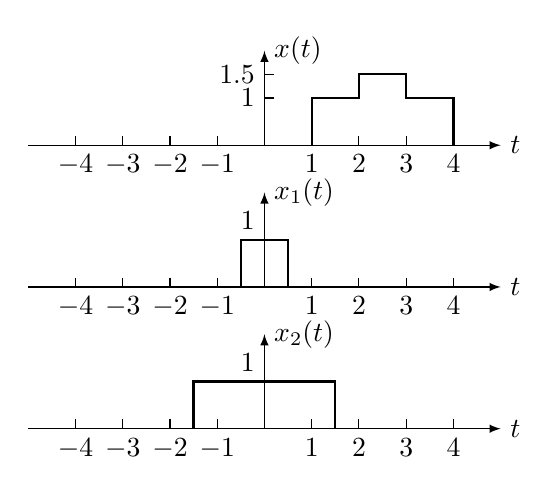
\begin{tikzpicture}[scale=0.6]
	\begin{scope}
		\def\xmin{-5}
		\def\xmax{5}
		\def\ymin{0}
		\def\ymax{2}
		
		\draw[-latex] (\xmin, 0) -- (\xmax, 0) node[anchor=west] {$t$};
		\draw[-latex] (0, \ymin) -- (0, \ymax) node[anchor=west] {$x(t)$};
		
		\foreach \x in {-4, -3, -2, -1, 1, 2, 3, 4}
		{
			\draw (\x, 0.2) -- ++(0, -0.2) node[anchor=north] {$\x$};
		}
		\foreach \y in {1, 1.5}
		{
			\draw (0.2,  \y) -- ++(-0.2, 0) node[anchor=east] {$\y$};
		}	
		\draw[thick] (1,0) |- (2, 1) |- (3,1.5) |- (4,1) -- (4,0);	
	\end{scope}
\pause
	\begin{scope}[yshift=-3cm]
		\def\xmin{-5}
		\def\xmax{5}
		\def\ymin{0}
		\def\ymax{2}
		
		\draw[-latex] (\xmin, 0) -- (\xmax, 0) node[anchor=west] {$t$};
		\draw[-latex] (0, \ymin) -- (0, \ymax) node[anchor=west] {$x_1(t)$};
		
		\foreach \x in {-4, -3, -2, -1, 1, 2, 3, 4}
		{
			\draw (\x, 0.2) -- ++(0, -0.2) node[anchor=north] {$\x$};
		}
		
		
		\node at (0,1) [anchor=south east] {$1$};		
		
		\draw[thick] (-0.5,0) |- (0.5, 1) -- (0.5, 0);	
	\end{scope}
	\begin{scope}[yshift=-6cm]
		\def\xmin{-5}
		\def\xmax{5}
		\def\ymin{0}
		\def\ymax{2}
		
		\draw[-latex] (\xmin, 0) -- (\xmax, 0) node[anchor=west] {$t$};
		\draw[-latex] (0, \ymin) -- (0, \ymax) node[anchor=west] {$x_2(t)$};
		
		\foreach \x in {-4, -3, -2, -1, 1, 2, 3, 4}
		{
			\draw (\x, 0.2) -- ++(0, -0.2) node[anchor=north] {$\x$};
		}
		
		
		\node at (0,1) [anchor=south east] {$1$};		
		
		\draw[thick] (-1.5,0) |- (1.5, 1) -- (1.5, 0);	
	\end{scope}
\end{tikzpicture} 